\documentclass{standalone}
\usepackage{ tikz }
\usepackage{ xparse }
\usepackage{../../../macros}

\begin{document}
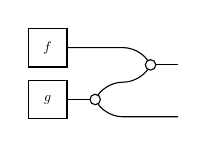
\begin{tikzpicture}[yscale=-1,x=1em,y=1.25em]

    \node (F) [draw, anchor=east, minimum size=1.4em, fill=white] at (0,0) {\scalebox{0.5}{$f$}};
    \node (G) [draw, anchor=east, minimum size=1.4em, fill=white] at (0,1.5) {\scalebox{0.5}{$g$}};

    \node (C1) [draw, circle, fill=white, scale=0.4] at (1,1.5) {};
    \node (C2) [draw, circle, fill=white, scale=0.4] at (3,0.5) {};

    \coordinate (X1) at (2,0);
    \coordinate (X2) at (2,1);
    \coordinate (X3) at (2,2);

    \draw (F) to (X1) to[out=0, in=255] (C2);
    \draw (C1) to[out=285, in=180] (X2) to[out=0, in=105] (C2);
    
    \draw (G) to[out=0, in=180] (C1);
    
    \coordinate (O1) at (4, 0.5);
    \coordinate (O2) at (4, 2);

    \draw (C2) to (O1);
    \draw (C1) to[out=75,in=180] (X3) to (O2);

\end{tikzpicture}
\end{document}